%update: Jan 13 gramma corrections undergoing...
%update: Jan 09-11 prof check
%update: Jan 03 rewrite all. 
%update: Dec 29 rewrite two parts. 
%update: Nov 21 citation done , figure done. 
%update: Nov 10 by zc, add more text(slightly edited), uploaded and compiled all figures. 
%update: Nov 09 by professor, rewrite the first half of text. 

%\begin{savequote}[75mm] 
%I am somewhat exhausted; I wonder how a battery feels when it pours electricity into a non-conductor?
%\qauthor{Sherlock Holmes (Arthur Conan Doyle)} 
%\end{savequote}

\chapter{\emph{In situ} TEM Electrical Probing for Ultrastable Sodium Ion Batteries}

\newthought{Sodium-ion batteries (SIBs)}, as an important alternative for future energy storage, have been on stage since 1980s. Among many anode materials, elemental phosphorus (P) has attracted most of the interest in recent years because of large theoretical capacity, i.e. 2596 mAh/g. The prime disadvantage, however, of a P anode is its poor conductivity and fast structural degradation due to volume expansion, as much as >490\%, over working cycles. To address this issue, I redesigned the anode structure via fabricating a flexible paper made of amorphous P and N-doped graphene. The as-fabricated anode delivers ultrastable characteristics and superb rate capability, 809 mAh/g at 1500 mA/g. The extraordinary structural integrity of this new anode was then studied via \emph{in situ} experiments inside a high-resolution transmission electron microscope (HRTEM), thereby the cyclic dynamics and sodiation/desodiation mechanisms were thoroughly understood. To confirm my experimental results, Density Functional Theory (DFT) calculations were additionally performed to indeed confirm that the N-doped graphene contributes to an increase in capacity for Na storage, and to an improved anode rate performance.

\section{Introduction}
Sodium ion batteries (SIBs) are receiving considerable attention and have bright expectations as one of the most promising alternatives to lithium ion batteries (LIBs) for energy storage.\cite{Ren2014c,Yang2011c,Liu2014a,Wen2014b,Shen2015b,wang2014e,Wu2014b,Yao2015b,Ni2014b} Both battery types possess analogous chemistry, but SIBs are cheaper because of more abundant sodium natural resources. In the recent reports, the cathode performance in SIBs was found to be comparable with that of the LIBs.\cite{Sun2014b,Barpanda2014b} However, the performance is still not good enough for the immediate practical applications. There have been an increasing interest in developing high-power and high-capacity anode materials for the next generation SIBs,\cite{Ong2011b,Palomares2012b,Zhu2014b,Yu2014b,Berthelot2011b,Qian2012d,Wang2013g,Komaba2011b,Cao2012b,Wang2013h,Xu2013b,Qian2012e} such as transition metal oxides,\cite{Zhu2014b,Yu2014b,Berthelot2011b} Prussian blue analogues,\cite{Qian2012d,Wang2013g} hard carbon materials,\cite{Komaba2011b}, nanowires,\cite{Cao2012b} graphene,\cite{Wen2014b,Wang2013h}, tin composite, \cite{Xu2013b} and antimony-based materials\cite{Qian2012e}, but their specific capacities are still not competitive for future applications(<800 mAh/g). \\

\begin{figure}  
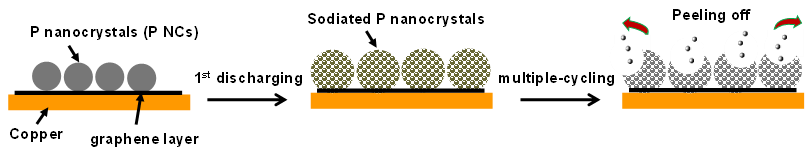
\includegraphics[width=\textwidth]{figures/figure4_s1}
\caption[Peeling off after cycling]
{Schematic diagram of the structural fracture of a high-volume-change type P anode, in which P nanocrystals anchored on the graphene layer are placed on the surface of a Cu current collector. After 1st discharging, there is a large volumetric expansion (>200-500\%) for P NCs; during cycling, such large volume change will lead to the pulverization and thus peeling off the electrode.
\label{fig:4_s1}}
\end{figure}

Among the hottest materials, elemental phosphorus (P) is one of the most attractive candidates with an ultra-high theoretical capacity of 2596 mAh/g\footnote{All capacities mentioned though the thesis are calculated based on the weight of composites.},\cite{Qian2013b,Kim2013c,Li2013c} i.e. about seven times higher than that of the commercial graphite anode in LIBs. The key challenge associated with a phosphorus anode is its rapid structural degradation caused by huge volume change (>490\%) under cycling. For conventional crystalline phosphorus (Figure \ref{fig:4_s1}), upon Na insertion, the P crystals are pulverized and thus the electrode film surface cracks (as a result of ~200-500\% volumetric expansion), leading to phosphorus peeling off from the current collector, which, in turn, gives a significant performance fading. So, stabilizing or sustaining the rigidness of the phosphorus anode structure during cycling is the practical key toward the improvement of the cycling performance of a P-based SIB anode. Very recently, notable breakthroughs have been witnessed in stabilizing anode structure through a design of amorphous P/carbon hybrids.\cite{Qian2013b,Kim2013c,Li2013c} For example, Qian et al. reported that the amorphous P/C hybrids prepared under high-energy mechanical milling had demonstrated a considerable capacity retention of 68\% after 60 cycles at the current density of 250 mA/g.\cite{Qian2013b} Kim et al. demonstrated that a similar amorphous P/C structure is able to deliver as high as 80\% reversible capacity and less than 7\% capacity fading after 30 cycles at a current density of 143 mA/g.\cite{Kim2013c} In addition, Chou et al. fabricated a composite anode via simple hand-grinding of commercial microsized red phosphorus and carbon nanotubes (CNTs); this demonstrated a high capacity retention of 76.6\% over 10 cycles.\cite{Li2013c} The improvements in cycling stability in the regarded reports were indeed remarkable, however, capacity retentions of less than 80\% still indicate that further developments are still needed in order to meet the practical requirements.\cite{Luo2015b}\\

\begin{figure}  
\centering
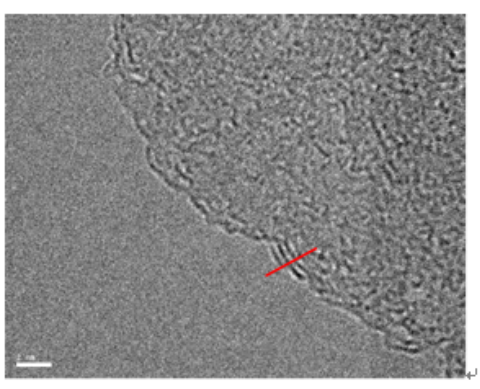
\includegraphics[width=300pt]{figures/figure4_s2}
\caption[TEM of GN]
{HRTEM image of an N-doped graphene (GN).
\label{fig:4_s2}}
\end{figure}

\begin{figure}  
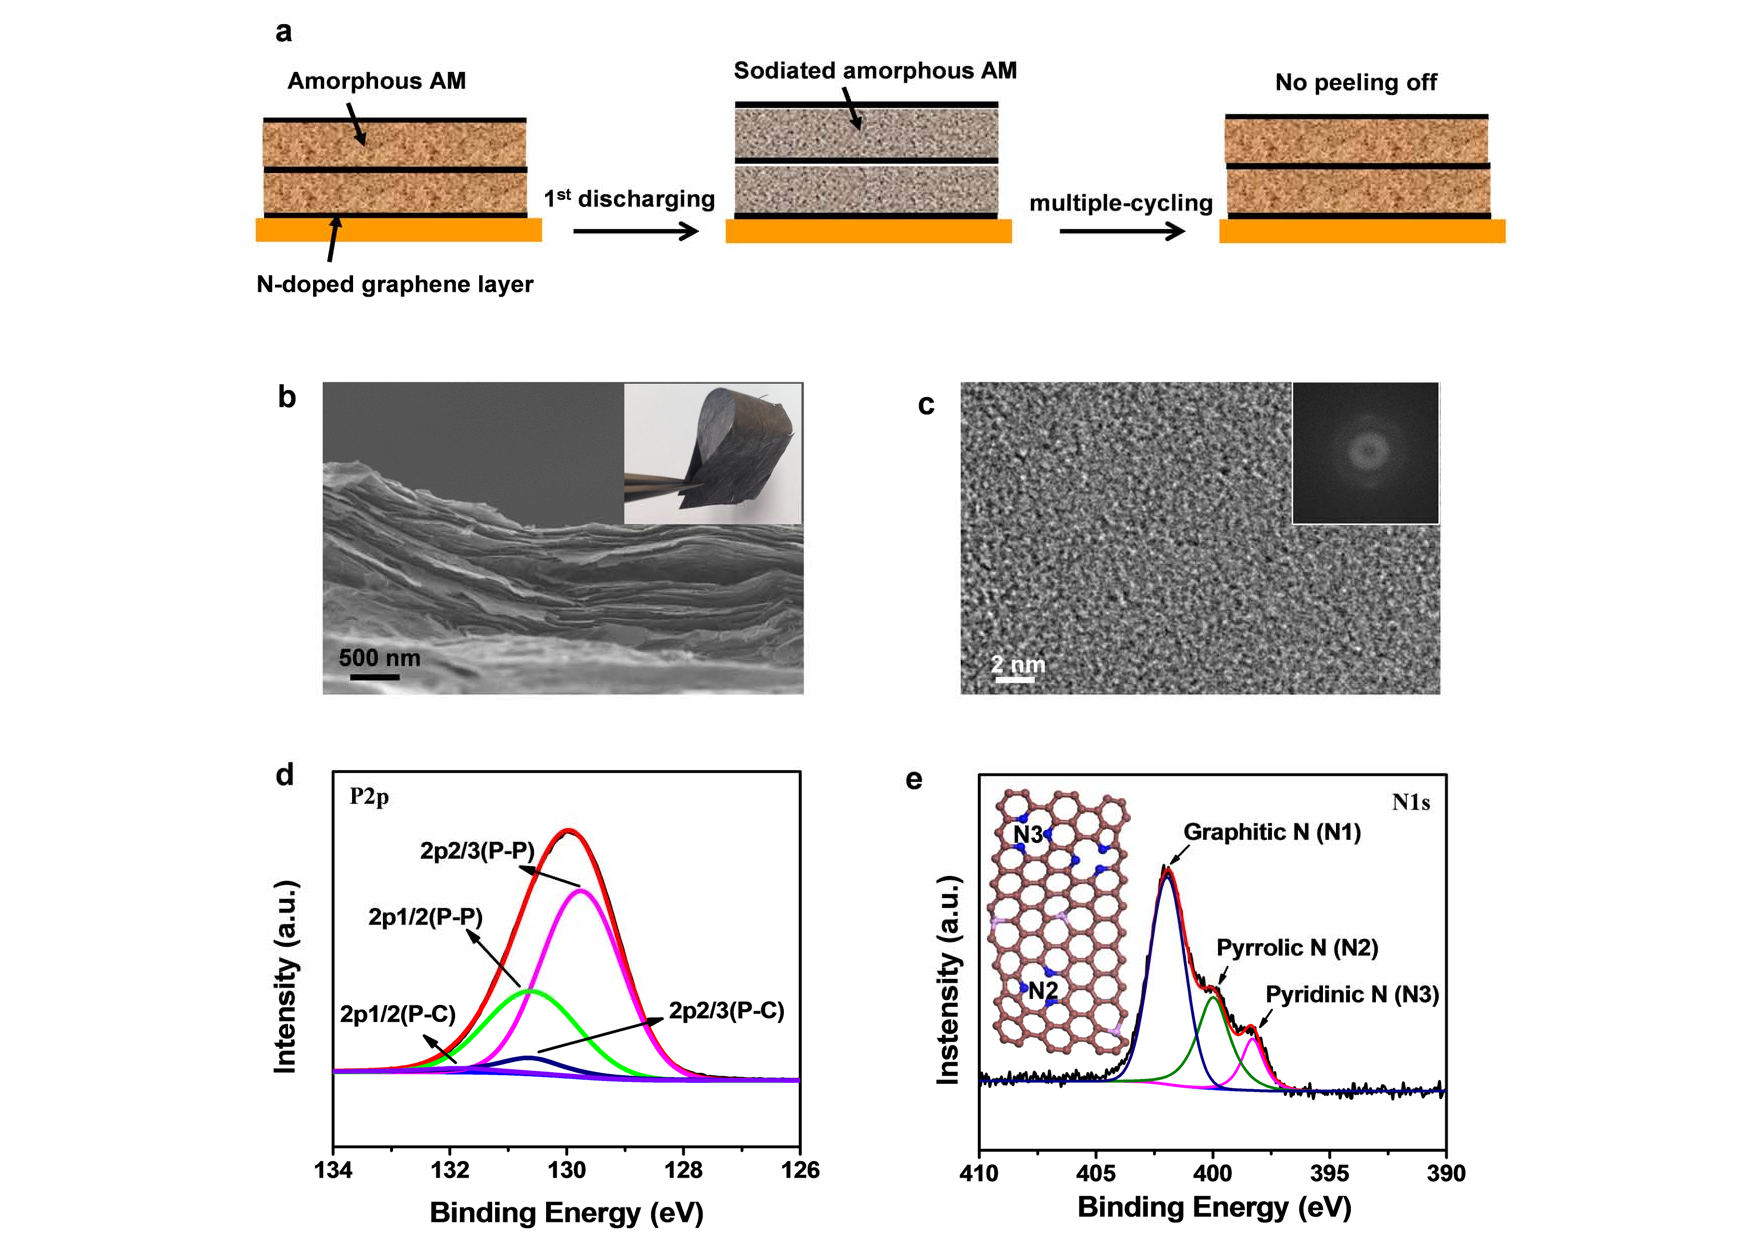
\includegraphics[width=340pt, angle=-90]{figures/figure4_1}
\caption[Layered structure design]
{(a) Illustrative scheme of the designed layered anode structure. (b) SEM image of the cross section of a P@GN paper, the inset shows its paperlike appearance. (c) HRTEM image and the corresponding FFT pattern of the P@GN portion confirming its amorphous structure. d-e) P2p and N1s XPS spectra of P@GN. N2 and N3 represent pyrrolic N and pyridinic N, respectively. 
\label{fig:4_1}}
\end{figure}

To obtain a stable P-based Na-ion battery anode having high capacity retention and rate performance, a flexible hybrid amorphous P-embedded N-doped graphene paper was designed and studied in my work. Unlike the standard methods which assemble the P and C components via any mechanical mixing (milling or grinding), a smarter design should tackle the existing problems, such as electrode chemical stability during sodiation-desodiation and mechanical robustness after hybridization. Therefore, a few-layered N-doped graphene (GN) (Figure \ref{fig:4_s2}) is herein selected as a substrate, whose two-dimensional (2D) nanosheet architecture provides a decent framework ensuring uniform deposition of amorphous P.\cite{Nicolosi2013b,Huang2015b} Several advantages associated with the designed amorphous P@GN hybrids (Figure \ref{fig:4_1}a) prepared by the developed so-called “phase-transformation” route are:\\
(1) Compared with crystalline P (Figure \ref{fig:4_s3}), amorphous P is more stable because of its relatively small volume change.\cite{Qian2013b,Kim2013c} Through the uniform confinement of the amorphous P within GN frameworks, the flexible GN can effectively buffer the volume change. This effectively prevents the electrode fracture and ensures the improvement of the battery capacity retention during electrochemical cycling;\\
(2) The possibly formed robust P-C bonds between P and GN layers anchor both components, serving like several elastic “springs” between them; this also helps to further enhance the stability of the anode;\\
(3) The GN nanosheets provide high conductivity electron transport networks and robust mechanical backbones, so that amorphous P could be very electrochemically active. In addition, the high tenacity of GN is useful to accommodate the volumetric expansion of P without mechanical damage or peeling off effects. Furthermore, N-doped graphene also contributes with a certain capacity to the SIBs and brings the fast sodium ion transport according to the DFT calculations.
Thus in this Chapter, I show that the above-mentioned three key features of the amorphous P@GN structure endows the large-volume-change anode with a superb capacity retention (>85\% over 350 cycles), outstanding cycle stability (0.002\% decay per cycle from 2nd to 350th cycle), and excellent rate capability (809 mAh/g at 1500 mA/g). Most importantly, state-of-the-art {\em in situ} probing experiments in HRTEM and supporting theoretical calculations finally uncover the key advantages of the present design and ensure the future developments of the P-based high-performance SIB anode structures, while getting deep insights into the associated atomistic mechanisms. 

\begin{figure}  
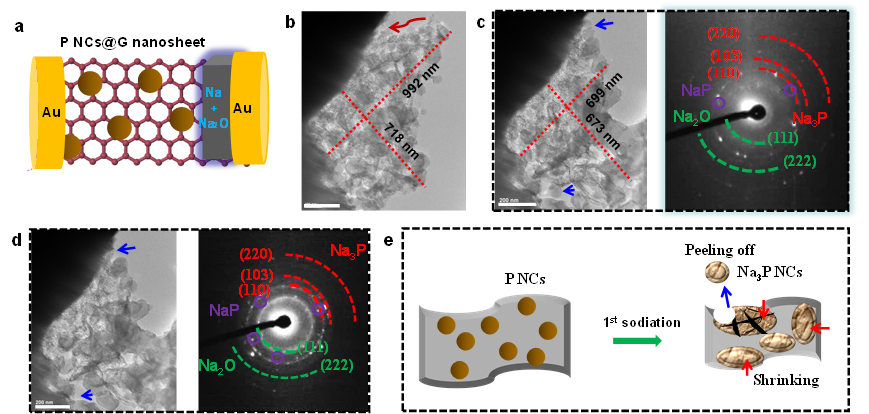
\includegraphics[width=370pt,angle=0]{figures/figure4_s3}
\caption[Layered structure design]
{a) Schematic illustration of an individual P nanocrystals@G (P NCs@G) nanosheet prototype sodium battery device fabricated under {\em in situ} TEM. b) TEM image of the nano-SIB at the initial stage. c-d) Time-dependent TEM images and SAED patterns of sodiated P NCs@G nanosheet upon sodiation at 5 s and 120 s. e) The schematic illustration of the 1st sodiation-desodiation process of P@GN nanosheet. Red arrows indicate the shrinkage, while blue arrows indicate particles peeled off. Scale bars: 200 nm. 
\label{fig:4_s3}}
\end{figure}

\section{Experimental}
%from main text.
Amorphous P@GN paper was prepared by a designed "phase-transformation" route. Bulk red P was heated to form P4 vapors in a sealed ampule, which were adsorbed and deposited within the inter-layers of GN; it changed back into amorphous red P after condensation.\cite{Roth1947b} Thus, a butter-bread-like structure composed of flexible conductive GN layers and thin amorphous red P layers between them was fabricated (Figure \ref{fig:4_1}b). 
%from SI.
Synthesis of P@GN: Graphene oxide (GO) suspension used in this work was prepared via a modified method. 50 mg of graphene oxide was loaded in a ceramic boat in a tube furnace followed by its heat treatment at 600 degrees Celsius for 1.5 hours in a gas mixture of NH3 and Ar (1:2 vol/vol) under a total flow rate of 150 ml/min. Commercial red phosphorus was dispersed in water and put into a Teflon-lined stainless autoclave. The autoclave was heated to 200 degrees Celsius and maintained for 12 h to remove surface oxides. As-prepared N-doped graphene (GN) products were properly mixed together with the pretreated red phosphorus powder, and sealed in an ampule in an inert Ar atmosphere. The sealed reactors were thermally treated at 500oC for 1 h and then at 280oC for several hrs in the furnace, before natural cooling to room temperature. The final product was washed with CS2, water and methanol, and then dried at 60oC.\\

Characterization: TEM images were taken with a 300 kV JEOL 3000F microscope. Samples were first dispersed in ethanol and then collected using carbon-film-covered copper grids. To avoid possible electron beam effects (such as radiolysis or sputtering damage of both Na-containing species and graphene lattice) the beam intensity was minimized. Scanning electron microscopy (SEM) images were recorded on a Hitachi S4800 electron microscope operating at 15 kV. XRD patterns were taken on a Philips X Pert PRO MPD X-ray diffractometer operated at 35 kV and 45 mA with Cu Kα radiation. XPS measurements were carried out on an ESCALab220i-XL spectrometer by using a twin-anode Al Ka (1486.6 eV) X-ray source. All the spectra were calibrated to the binding energy of C 1s peak at 284.6 eV. The background pressure was ~3 x 10-7 Pa. Raman spectra were collected on a Horiba Jobin-Yoon T6400 Raman spectrometer.\\
Electrochemical tests: The electrochemical properties of P@GN and P NCs@G samples were studied using a 2032-type coin cell on a Hokudo Denko Charge/Discharge apparatus. The working electrode was prepared by directly pressing a piece of sample onto the Cu mesh current collector. Na metal foil was selected as the reference and counter electrode. The electrolyte was 1 M NaPF6 in ethyl carbonate (EC) and diethyl carbonate (DEC) ($EC : DEC = 1 : 1 vol/vol$). The cells were assembled in a glove box filled with a pure argon gas.\\ 
Construction of individual prototype P@GN (P NCs@G)-based SIB. In situ TEM observations were conducted in a JEOL-3100 FEF equipped with an Omega filter and a {\em Nanofactory Instruments} STM-TEM holder. In order to build up the test cell, an individual P@GN or P NCs@G nanosheets were attached to the fresh-cut flattened Au wire, which was then attached to the piezo-manipulator. A small piece of Na foil was placed to another Au wire as a reference and counter electrode. Before insertion of the holder into the TEM column, a piece of Na foil covered with a Na2O layer was placed on the surface of metal Au tip. Then isolated P@GN or P NCs@G samples were chosen for direct electrochemical tests. Under the following delicate piezo-driven TEM mechanical manipulations the two electrodes were connected and the probe cell was finally constructed. The sodiation was carried out at a negative bias in the range of -2 V to 0 V with respect to the Na metal.\\
DFT calculations. The first principle calculations were carried out using the Vienna ab initio simulation package (VASP),\cite{Kresse1996} where projected-augmented-wave (PAW) potential was adopted.\cite{Kresse1999} The functional of Perdew, Burke, and Ernzerhof (PBE) and the generalized gradient approximation (GGA)\cite{Perdew1996} were employed in the calculations. We used a $3\times3\times1$ mesh in the irreducible Brillouin zone for structure relaxation and $6\times6\times1$ mesh for self-consisted calculations. In all the calculations the forces were relaxed to the values lower than 0.02 eV per angstrom.

\section{Results and disscussions}

%text above is edited by prof on Nov9. 
%the following part is added on Nov10, which is rephrased by zc on Dec 29.

\begin{figure}  

\includegraphics[width=\textwidth]{figures/figure4_s4}
\caption[TGA curve of P@GN]
{TGA curve of P@GN sample.
\label{fig:4_s4}}
\end{figure}

It is considered that some P-C bonds possibly exist between amorphous P and GN layers which would tightly anchor those layers. Scanning electron microscopy characterization (Figure \ref{fig:4_1}b) illustrates the cross section of the structure of anode, where we can see a lot disordered and flexible layered structures. It is considered that most GN sheets can not be tranfered back to graphite by restacking even under longtime heating or mechanical induced compression.\cite{Huang2015b} From HRTEM image and the corresponding fast Fourier transform (FFT) patterns, crystallography of P is amorphous as depicted in Figure \ref{fig:4_1}c. We are able to observe the disordered nature of P@GN of structure from the diffused rings and the absence of all contrast due to lattice fringes. 

\begin{figure}  
\centering
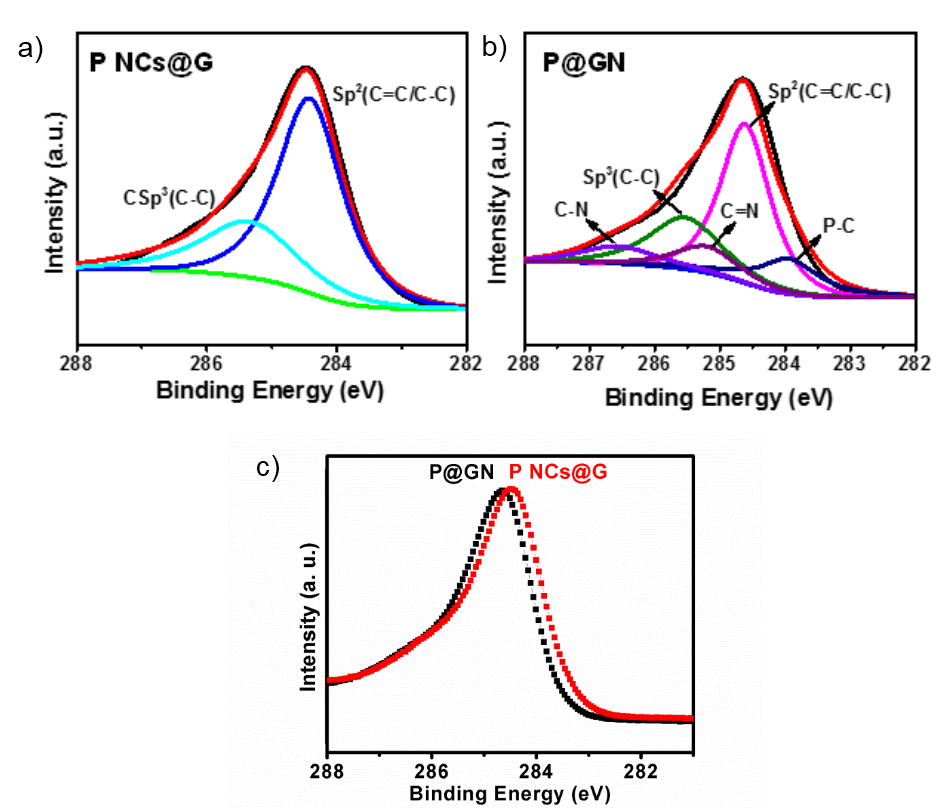
\includegraphics[width=320pt]{figures/figure4_s5}
\caption[C1s XPS spectra comparison]
{a-b) C1s XPS spectra of PNCs@G and P@GN samples. c) Overlay overlay of the two surveys for C1s spectra of the two samples. 
\label{fig:4_s5}}
\end{figure}

The constitution of P in the composite was characteried to be ~66\% by thermogravimetric analysis curve as shown in Figure \ref{fig:4_s4}. In Figure \ref{fig:4_1}d, the P2p X-ray photoelectron spectroscopy (XPS) fit 2p1/2 and 2p3/2 doublets, where two peaks at 129.75 eV (2p3/2) and 130.6 eV (2p1/2) suggest the possible existance of P-C bonding.\cite{Jiao2014b,Niu2014b,Zhang2013b} 

According to theoretical simmulations,\cite{Sun2014b,Claeyssens2009b} among all P-C bonding types -- sp3, sp2 in plane, sp2 at edge, and sp2 in aromatic ring -- the most stable one is the sp2 hybridized P-C bonds in aromatic ring because of bond length in the \pi-p* conjugation plane is the shortest. As the inset image illustrates in Figure \ref{fig:4_1}e, GN would provide sp2 P-C bond at edge and or at aromatic rings. In addition, more evidence from C1s XPS spectra as shown in Figure \ref{fig:4_s5} depicts the possibly existed P-C bonds are observed in P@GN. In order to get clear comparison, P nanocrystlas in pure graphene (this sample name will be short as P NCs@G) sample was also prepared for test. As shown in Figure \ref{fig:4_s5}a, clearly, there is no P-C bond found in P NCs@G. 

As compared with the sample set of P NCs@G, the sp2 carbon atom fraction decreases while sp3 C-C (285.3 eV) bonds prevail in P@GN (Figure \ref{fig:4_s5}b) possibly due to some defects caused by nitrogen doping. Three N-doping types are characterized to exist in P@GN (Figure \ref{fig:4_1}e): graphitic, quaternary N (N1, 401.7 eV), pyrrolic N (N2, 400.2 eV), and pyridinic N (N3, 399.1 eV).\cite{Roth1947b,Wang2012e,Wang2014f,Wang2013i} The N2 and N3 dopants are generally acknowledged to be located at the edges or surface defect sites such as vacancies.\\

\begin{figure}  
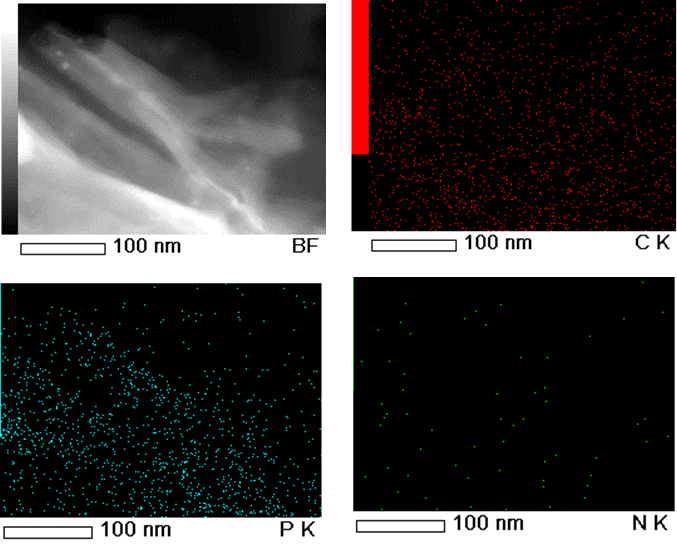
\includegraphics[width=\textwidth]{figures/figure4_s7}
\caption[Elemental maps of P@GN]
{
HAADF-STEM image, and C-, P- and N-elemental maps of a P@GN nanosheet. 
	
\label{fig:4_s7}}
\end{figure}

The specially designed layere structure exhibits revolutionary electrochemical performances. In Figure \ref{fig:4_2}, the battery performances of the P@GN were evaluated by using standard CR2032 coin cells. 

As comparison sample set, red P nanocrystals (NCs) placed on pure graphene (P NCs@G) were also manufactured by grinding of nanoscal red phosphorus and graphene. As shown in Figure \ref{fig:4_2}a, the initial Coulombic efficiency of P@GN is 87\%, higher than a that of 85\% for a reported P@C hybrid electrode.\cite{Li2013c} 
From the 2nd to 120th cycles at 200 mA/g or 350th cycle at 800 mA/g, the Coulombic efficiencies are more than 98\%. A discharge plateau as dipicted in Figure \ref{fig:4_2}b corresponds to an anodic peak starts from 0 V to 0.5 V, implying the formation of \ce{Na3P} with theoretical capacity of 2596 mAh/g. The conversion chemical reaction from P to \ce{Na3P} takes place. 
The chemical reaction process is then eventually proved by {\em in situ} HRTEM experiments which will be discussed in the following paragraphs. In reversed scan, a main anodic peak appears at 0.53 V, which possibly matches to a main sodium ion de-intercalation process of chemical reaction from Na3P to P. However, no clear peaks at any other potentials (for instance 0.63 V assigned to NaP) was found. This indicates that this electrode probably experience a reversible discharging/charging chemical cycling between \ce{Na3P} and P and affords very high capacity because of existence of \ce{Na3P}. \\

\begin{figure}  
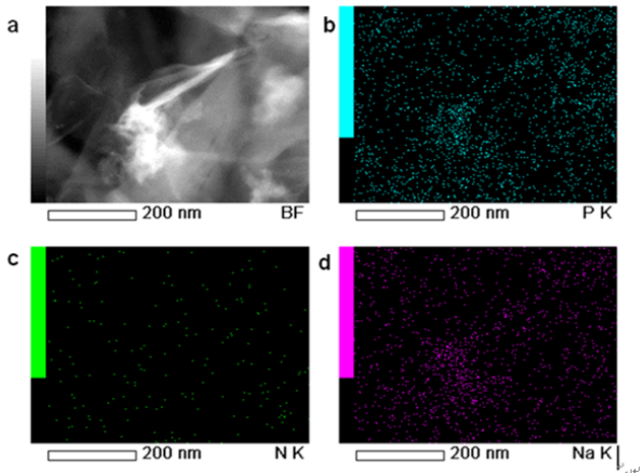
\includegraphics[width=\textwidth]{figures/figure4_s8}
\caption[Elemental maps of P@GN after 150 cycles]
{
The HAADF-STEM image and the corresponding elemental maps of a P@GN nanosheet at the fully desodiated state after 150 cycles.
	
\label{fig:4_s8}}
\end{figure}

Over 350 battery cycles, the capacity retention of P@GN battery is more than 85\%. From the 2nd to 350th cycle at 200 mA/g, the capacity decay is even less than 3\%. 
The excellent capacity retention and stability (about 0.002\% decay per cycle) are among the best cycling stablity performances of all reported P-based anodes to date. 
To reveal the mechanism of the unusual cyclic stablity, the original and after-cycled P@GN electrodes were examined by a high angular annual dark field (HAADF) imagine in scanning TEM (STEM) mode with the EDS mapping as illustrated in Figure \ref{fig:4_2}c, Figure \ref{fig:4_s7} and Figure \ref{fig:4_s8}. 
Obviously, integrity of the battery structure is maintained quite well in the desodiated states after even 120 cycles. 
It is also noted that upon sodiation, distribution of sodium species is very homogeneous over all nanosheet (Figure \ref{fig:4_2}c), this suggests the successful intercalation of sodium ions. 
The reduced volume expansion of P layers are significantly buffered and confined by GN layers, which is the key for refraining failure of anode structural. 
Moreover, P@GN anode material exhibits improved rate capability as compared with P NCs@G material, which are listed in Figure \ref{fig:4_2}d. 
At high current rate (1500 mA/g), the reversible capacity still reaches 809 mAh/g for P@GN. This capacity is twice higher than that of the theoretical capacity of commercial graphite (370 mAh/g) in LIBs. And, of course, these results are far better than those of the P NCs@G (~10 mAh/g at 1500 mA/g). \\
This is especially meaningful for future secondary battery choice. Sodium batteris are expected to be low cost with high capacity. 

%following part is now reprased by zc on Dec 30. 

\begin{figure}  
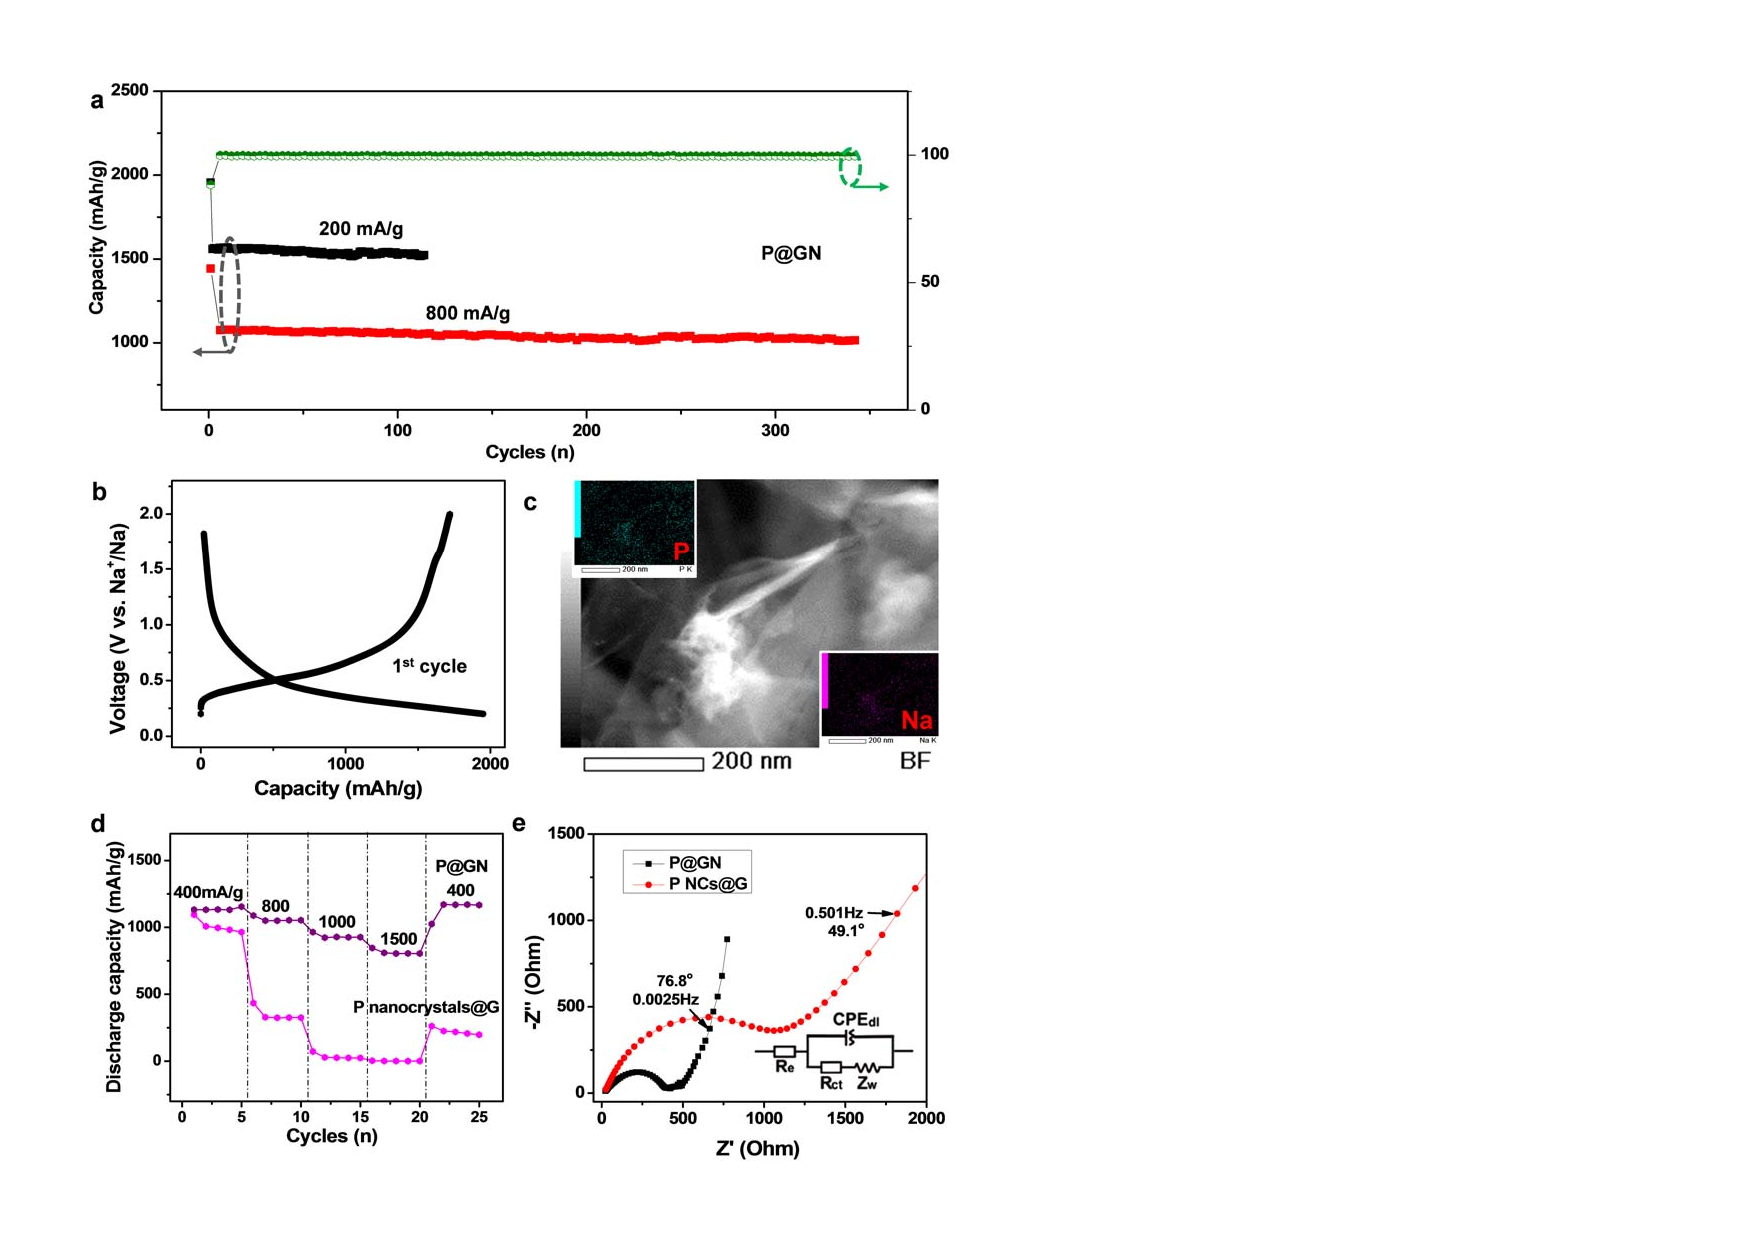
\includegraphics[width=400pt,angle=-90]{figures/figure4_2}
\caption[Performance of P@GN SIB]
{
(a) Cyclic capacity and Coulombic efficiency of P@GN at 200 mA/g and 800 mA/g. (b) Galvanostatic charge and discharge profile of P@GN anode at 200 mA/g. (c) The HAADF-STEM image and the corresponding EDS maps of a P@GN nanosheet at the desodiated state (after 120 cycles). (d) Rate capabilities of P@GN and P NCs@G. (e) Nyquist plots and equivalent circuit model of P@GN and P NCs@G electrodes after 10 cycles at 0.1 A/g in the discharged state. 
	
\label{fig:4_2}}
\end{figure}

To compare the battery anode kinetics of P@GN and P NCs@G, their electrochemical impedance spectroscopy (EIS) was performed as ploted in Figure \ref{fig:4_2}e. The Nyquist curves demonstrate that a diameter of the semicircle for P@GN anode material in high-medium frequency region is much less than that of P NCs@G electrode. This suggests that P@GN anode possess lower contact and better charge-transfer impedance. Based on the modified Randles equivalent circuit, shown in the inset of Figure \ref{fig:4_2}e, the P@GN anode exhibits a significant lower charge-transfer resistance. Therefore, P@GN holds a high electrical conductance and also provides more stable surfaces such as SEI layer. This leads to the better rate capability and reversible capacity as comparison with P NCs@G. 
In addition, the angle of low-frequency slope for P@GN (76.8 degrees) is steeper than that of P NCs@G (49.1 degrees), indicating higher diffusivity of \ce{Na+} for sodium ion uptake and extraction in P@GN anode due to the steep low-frequency tail.\cite{Sun2014b} \\

\begin{figure}  
\centering
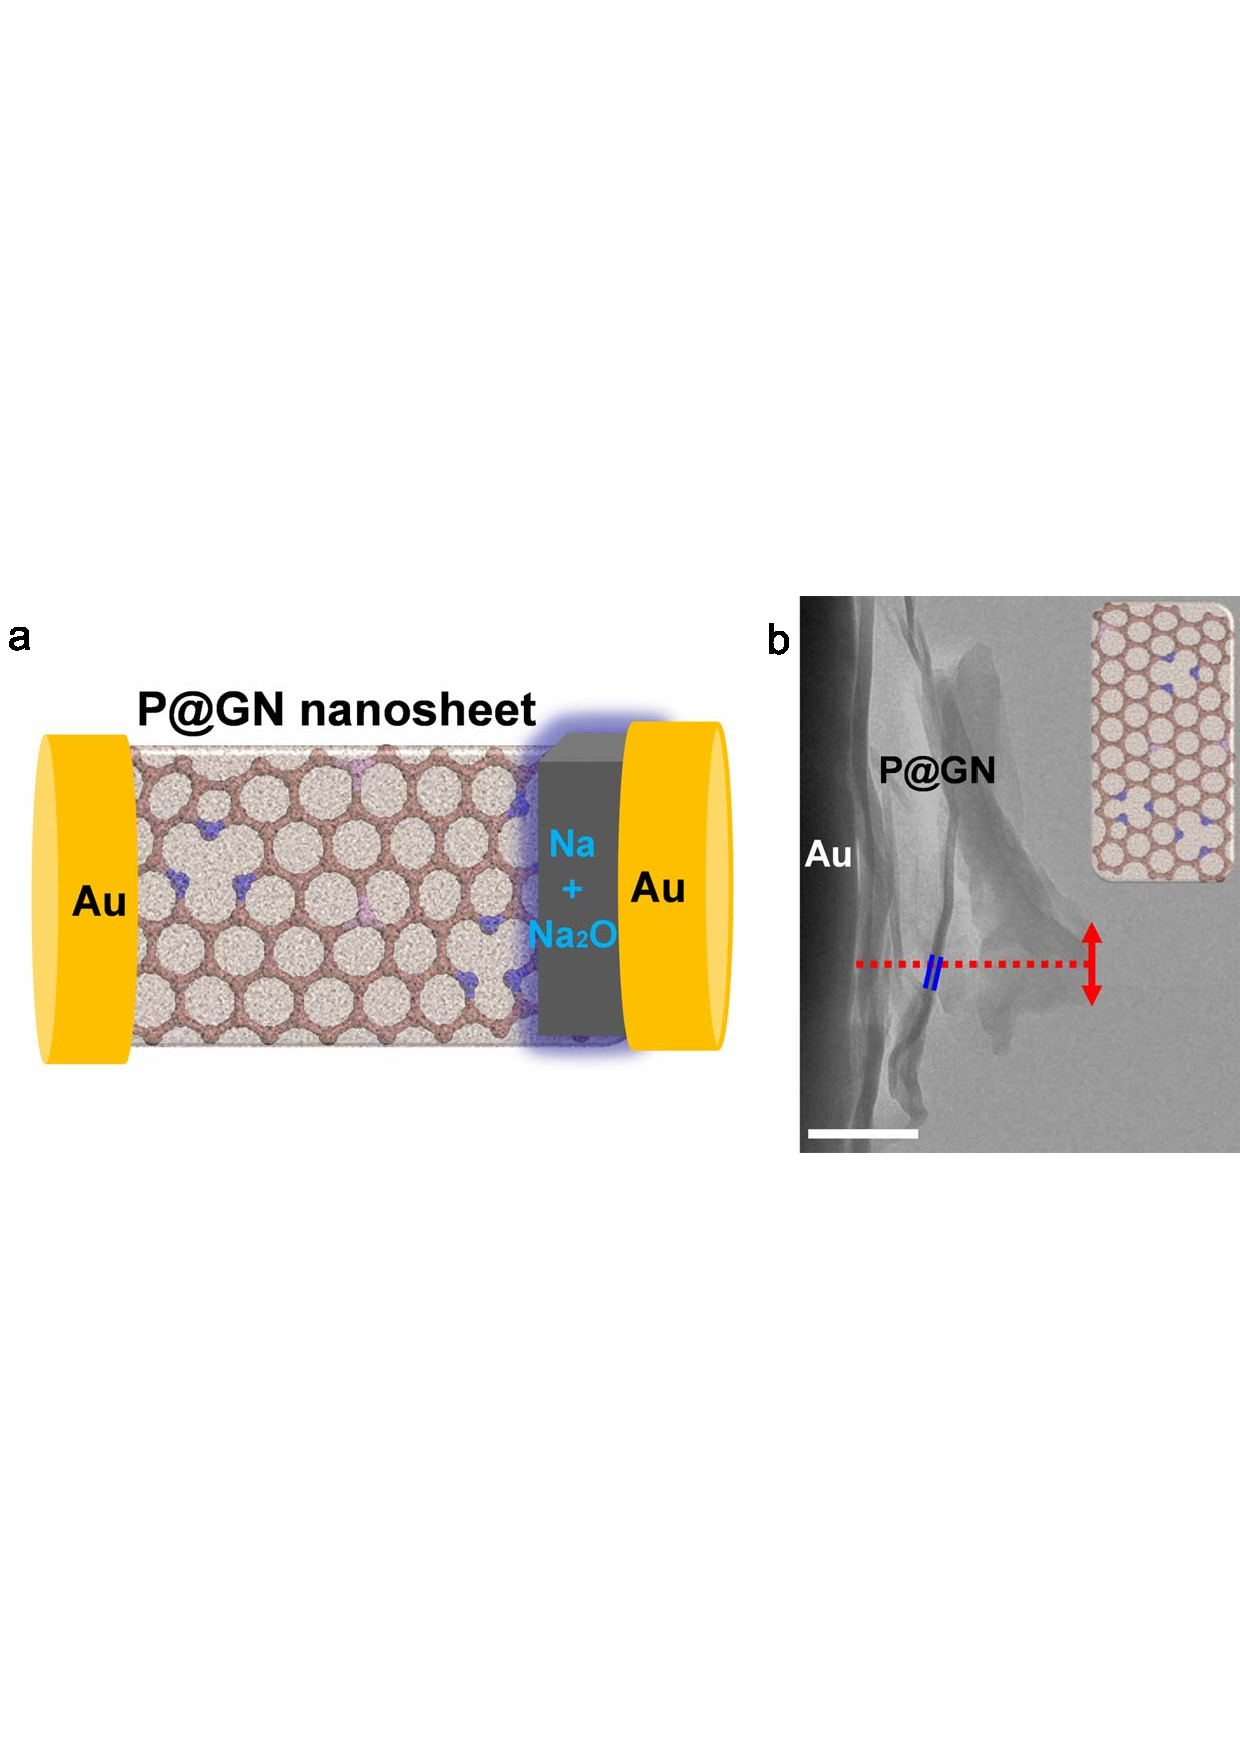
\includegraphics[width=300pt,angle=0]{figures/figure4_3ab}
\caption[{\it In situ} probing on P@GN SIB setup]
{
(a) Schematics of an individual P@GN nanosheet sodium ion battery device test performed by {\em in situ} TEM. 
(b) TEM image of the SIB at initial stage. Scale bars: 100 nm.
\label{fig:4_3ab}}
\end{figure}

It is very important to maintain the structural integrity during cycling to realize stable performance for large capacity and low-cost anode material.\cite{Liu2014a} 
To research mechanism of the anode stability of our ultra-stable decice, I performed an {\em in situ} TEM study of the chemical and structural changes of the as-fabricated anode during electrochemical cycling (Figure \ref{fig:4_3ab}). The {\em in situ} TEM experimental set-up is very similar to some previous reports (Figure \ref{fig:4_3ab}a).\cite{Wang2014f,Wang2012g} 
The setup mainly consists of two parts: the sample is on a gold wire tip, while another gold wire with a small piece of sodium is on the opposite side. Special care is required for sodium loading. Sodium is loaded to the probe (which is on the TEM holder) in glovebox with argon atomosphere. Then the holder was capped with argon. A few seconds before insertion of holder, the cap was removed. 
For transferring process, a very thin layer of \ce{Na2O} was formed on the sodium metal surfaces. The \ce{Na2O} layer serves as natural solid electrolyte for the single nanostructure SIB. Figure \ref{fig:4_3ab}b depicts a TEM image of a freestanding P@GN nanosheet material. 

\begin{figure}  
\centering
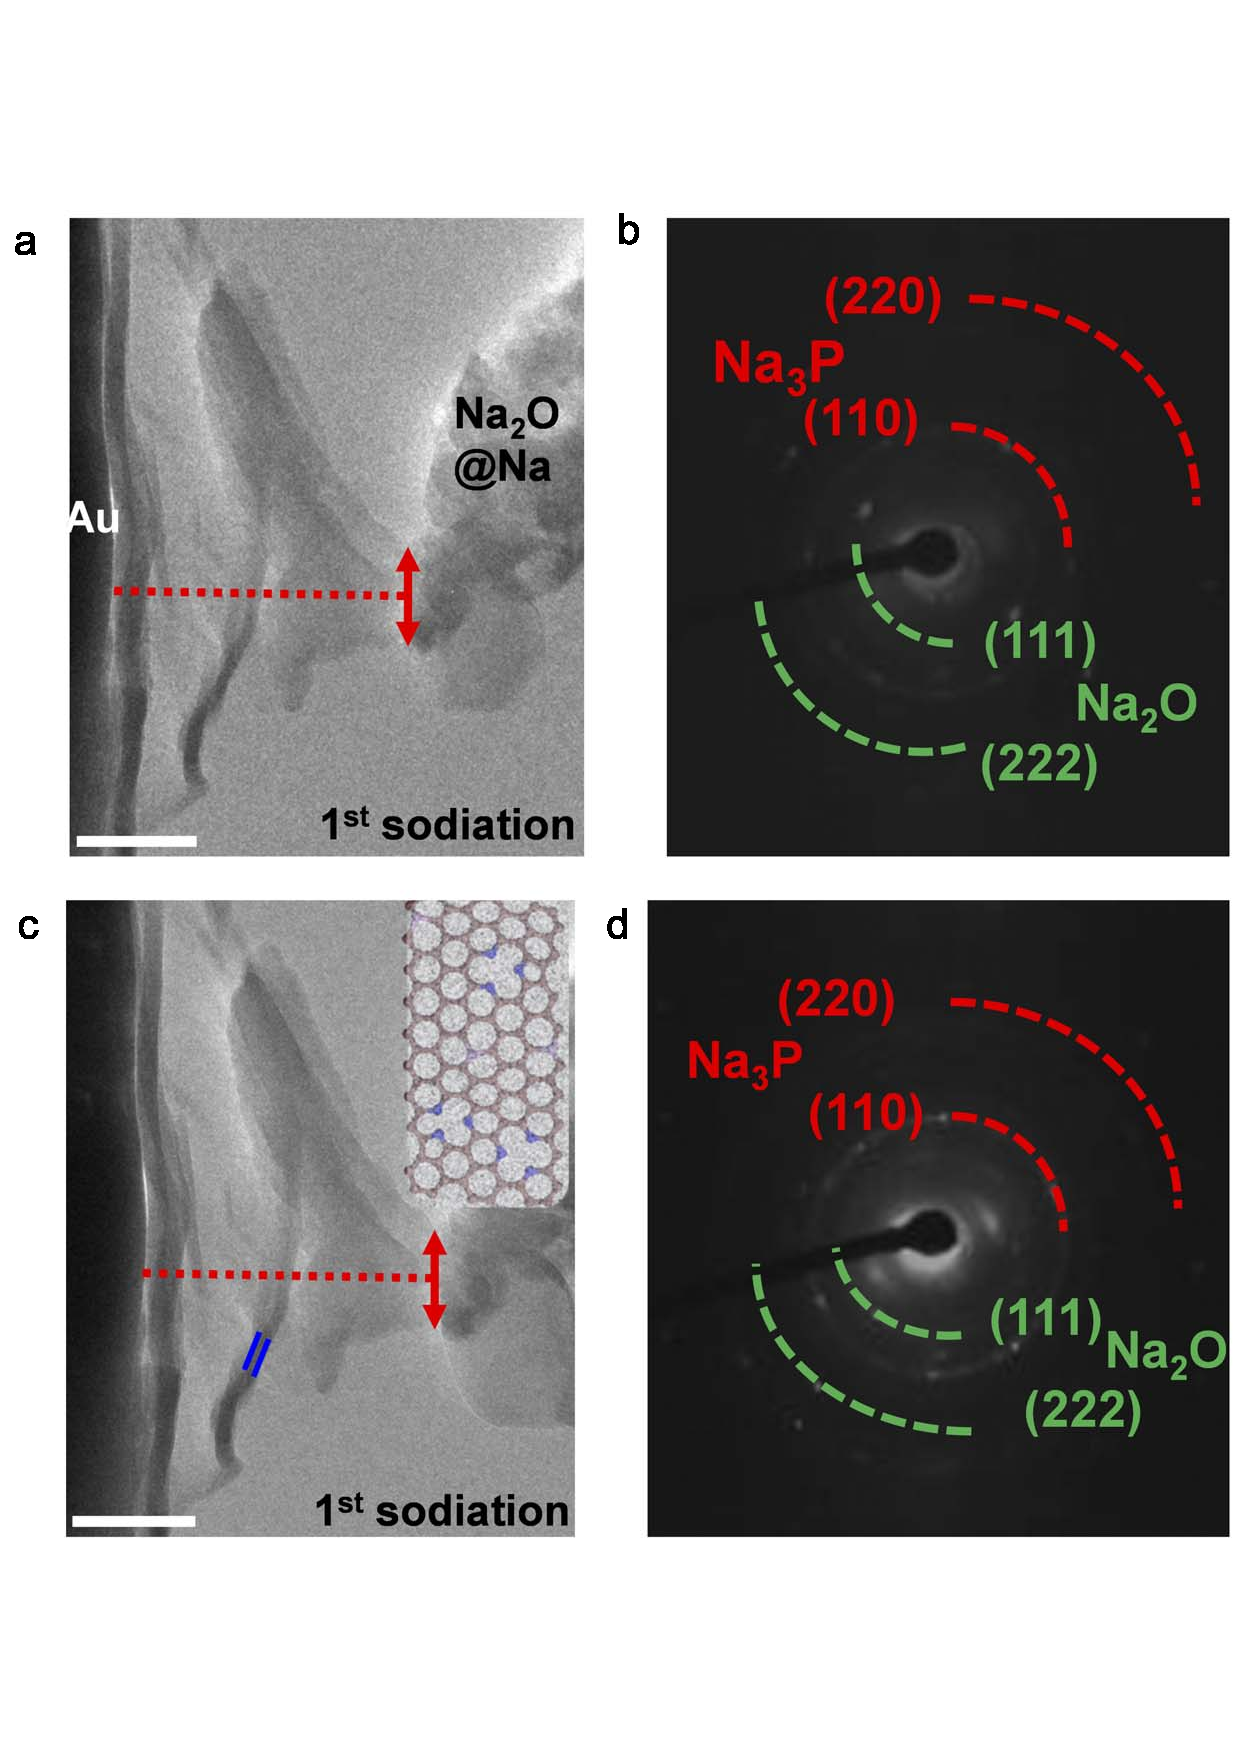
\includegraphics[width=320pt,angle=0]{figures/figure4_3cd}
\caption[{\it In situ} sodiation process of P@GN SIB]
{
 TEM image and SAED pattersn of the {\em in situ} SIB at (a) 15 s and (b) 120 s of sodiation during first discharging. Scale bars: 100 nm.
\label{fig:4_3cd}}
\end{figure}

Figure \ref{fig:4_3cd} present the sodiation process of an individual P@GN anode.
A -2 V potential was applied to P@GN anode with respect to the sodium potential.
The anode material immediately expanded in both longitudinal and transverse directions after the applying of bias, as shown in Figures \ref{fig:4_3cd}. 
After sodiation, the length of nanosheet increased from initial 210 nm to the sodiated 250 nm, and the length of a regional edge enlarged to 83 nm from previous 65 nm. 
The experiment further implies that an effective Na transport along/across the hybrid structure indeed took place. 
It is noted that the expansion rate in the one direction, from 210 nm to 250 nm, becomes less than that for another one, from 65 nm to 83 nm. This might indicate small-sized nanoribbons could process higher electrochemical activities. 
No significant evidence of structural degradation was found even after entire sodiation (Figure \ref{fig:4_3cd}b). This is confirmed by the decent flexibility of GN and amorphous P layer which can effectively buffer large volume expansions during insertion of sodium ions. 
The nanosheet thickness also increased from 10 nm to 14 nm as is marked by blue color in Figures 3b and  3d during discharg process. 
The SAED pattern of the sodiated P@GN (Figure \ref{fig:4_3cd}) reveals the crystallography information of phase changes aftersodiation. 
The main phase of the sodiated anode material is identified to be \ce{Na3P} -- which takes more sodium ions than \ce{NaP} for a single P atom. This result is consistent with the battery test as shown in Figure \ref{fig:4_2}b. 

\begin{figure}  
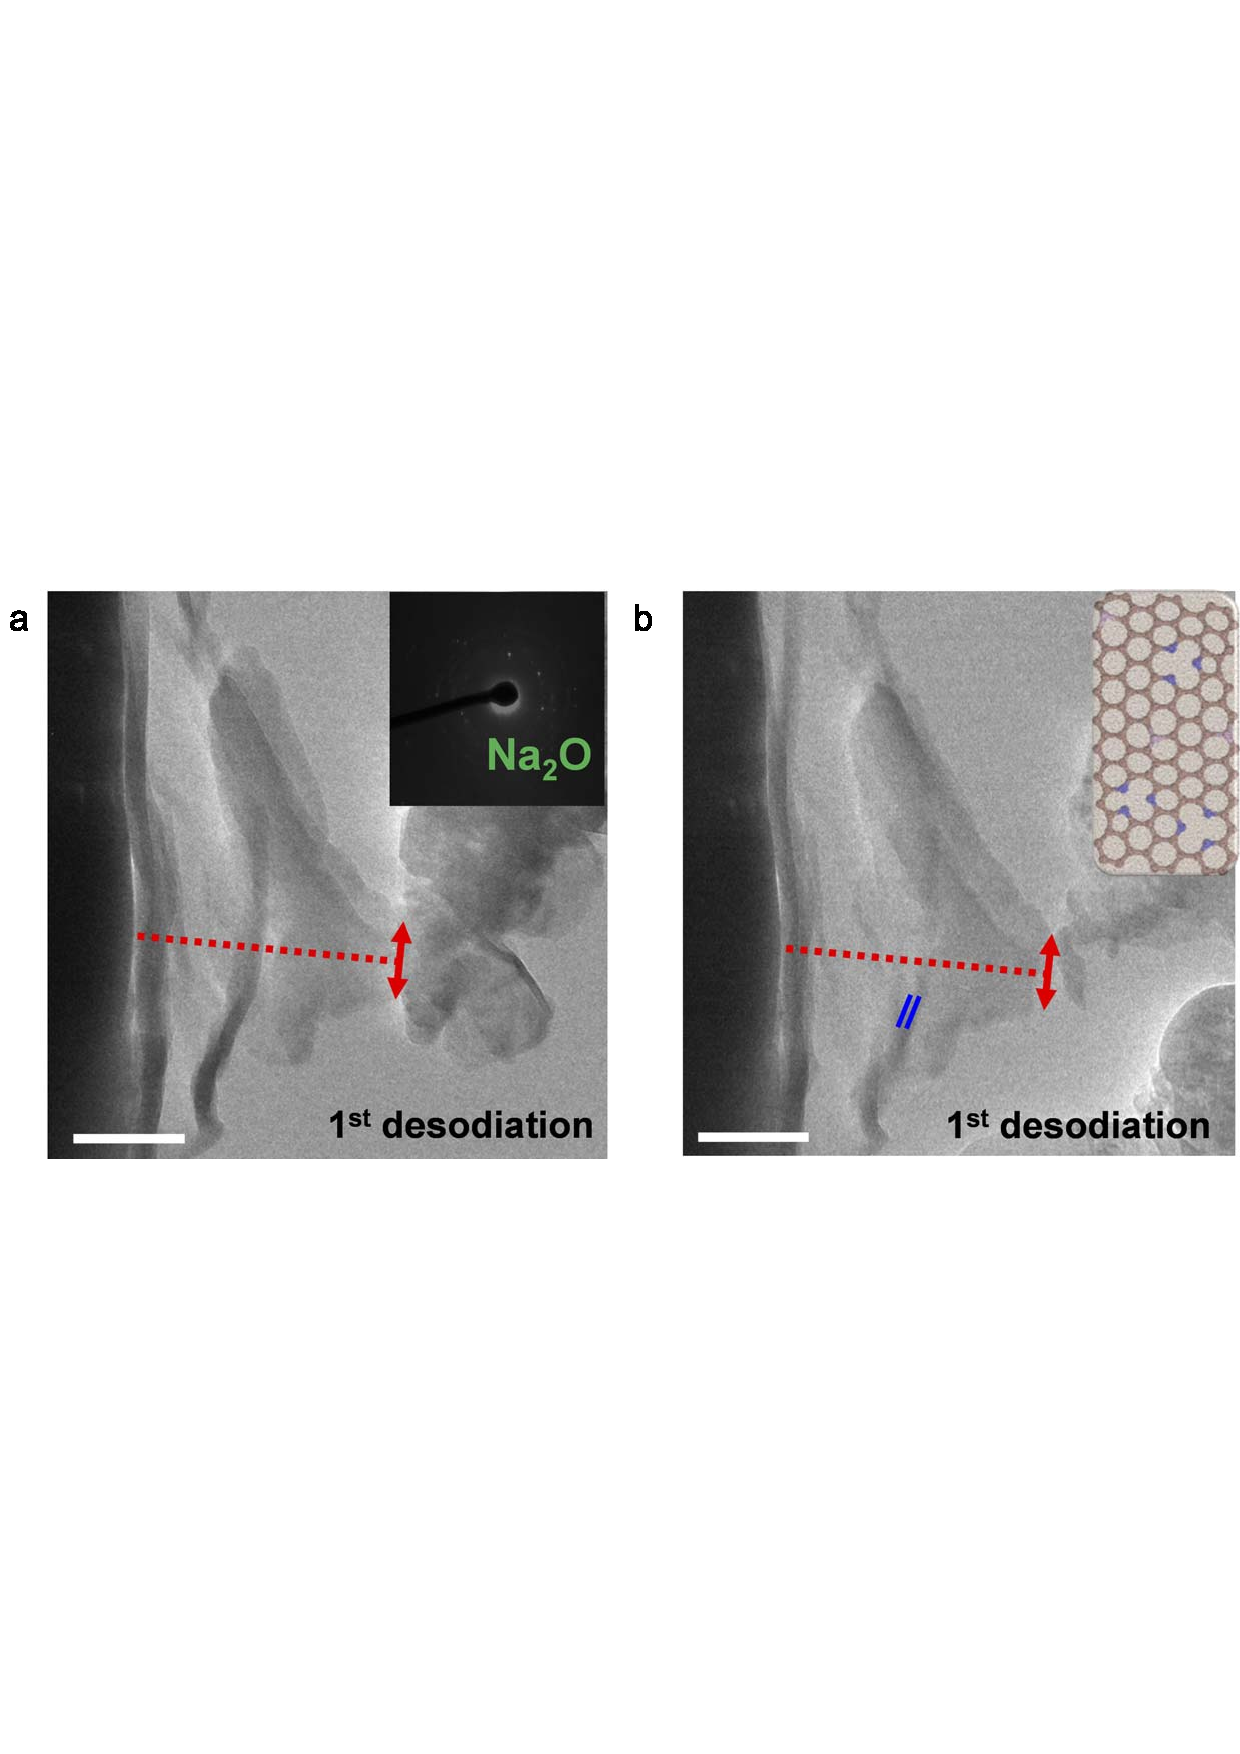
\includegraphics[width=\textwidth,angle=0]{figures/figure4_3ef}
\caption[{\it In situ} desodiation process on P@GN SIB]
{
  (a) 5 s and (b) 120 s of time-dependent TEM images of desodiation during 1st charging. Insets show the corresponding schematic atomic structures. The inset in (a) depicts the corresponding SAED pattern. Scale bars: 100 nm.
\label{fig:4_3ef}}
\end{figure}

%this part is rephrased by zc on Jan 2. 
The desodiation process took place when 2 V bias was applied to the nanostructure. As presented in Figure \ref{fig:4_3ef}, the volume shrinkage became observable along both longitudinal and transverse directions. 
It is observed that desodiated nanosheet after sodium extraction looks quite similar to the initial shape. What's more, the edge segment perfectly kept the pristine state. 
The experiment demonstrates that the designed layerd structure denotes to buffer the anode volume expansion and shrinkage during electrochemical cycling. 
Therefore, the {\em in situ} experiments explain the stable cycling performance as shown in the {\em ex situ} battery measurements (Figure \ref{fig:4_2}b). 
Integrity of P@GN nanosheet is preserved quite well, suggesting that the butter-bread-like structure are effective for relaxing strain and overcoming pulverization caused by volume expansion, and in hence it can be a very promising anode candidate for SIB.\\

The comparison material, indicidual P NCs@G nanosheet, was also build and tested by {\em in situ} microscopy. 
As shown in Figure \ref{fig:4_s3}, during discharging, P nanocrystals expanded immediately. 
The whole P NCs@G nanosheet drastically shrinks instead of expanding upon sodium insertion along all directions, because the sodiated crystals aggregated together and also its size grew larger caused by Ostwald ripening.
Therefore, the large adhesive force between graphene and P NCs compressed all structure into a aggregate form of P NCs. 
Note that the phenomenon is more significant at the edge as compared with the basal plane due to higher electrochemical activities of the edges. 
Moreover, peeling off of active material can also be observed during {\em in situ} TEM process which is marked by blue arrows in Figure \ref{fig:4_s3}c-d. Two particles in the upper part and another nanocrystal in the lower part dissapeared after sodiation. 
The peeling off of active material implies that the P NCs@G experienced significant expansion, which leads to irreversable peeling off, and in hence caused a loss of capacity. 
It is noted that some NaP phases are shown in SAED patterns in Figures \ref{fig:4_3cd}, in the desodiated material. The NaP phases (instead of \ce{Na3P}) implies that only conversion of P into NaP rather than Na3P takes place. We know that \ce{Na3P} holds much higher capacity as 2569 mAh/g than that of NaP, which is only 856 mAh/gh. 
Sodiation of phospherous in P NCs@G sample can be associated with its low electrical conductivity and large crystal size. 
Therfore, the irreversible structural failure and the presence of NaP (instead of \ce{N3P}) undoubtedly limit the performance for P NCs@G. 
The {\em in situ} experiment is consistent with the battery cycling performance and rate properties (Figure \ref{fig:4_2}c). \\

\begin{figure}  
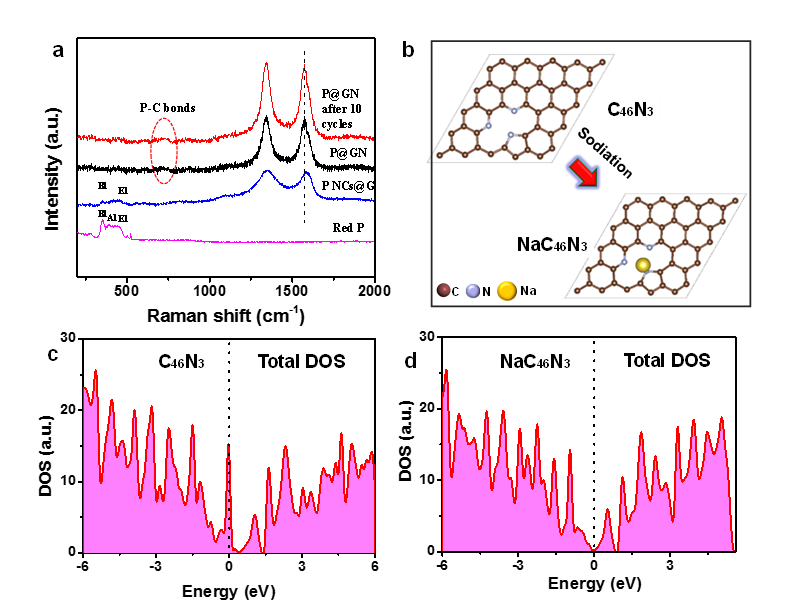
\includegraphics[width=\textwidth]{figures/figure4_4}
\caption[Raman spectra and DFT calculations]
{
(a) Raman spectra of red P, P NCs@G, and P@GN before and after sodiation. 
(b) The schematics of the insertion of sodium into a \ce{C46N3} sheet based on DFT calculations. 
(c-d) DOS of \ce{C46N3} and its sodiated product \ce{NaC46N3}.
\label{fig:4_4}}
\end{figure}

It is believed that maintaining amorphous morphology of P during cycling is a key factor for ultrastable battery performance. 
This is confirmed by the Raman spectroscopy presented in Figure \ref{fig:4_4}a. 
Spectrum features of red P between $300-500 cm^{-1}$ can be attributed to P–P stretching bonds of P9 and P7 cages to establish pentagonal tubes in paired layers.

%Rewrite rest part on Jan 03 by zc. 
Compared with red P material, the amorphous phosphorusi and nitrogen doped graphene hybrid structure does not display Raman peaks natural for P, but show two typical D-band and G-band peaks (peculiar to graphene).\cite{Kim2013c} 
The result indicates that the layerd P@GN paper was maintained during cycling. 
Additionally, Raman spectra of various samples provide more evidences for existence of the stable P-C bonds after multiple cycles. 
In Figure \ref{fig:4_4}a, a broad envelope centered at about $700 cm^-1$ for P@GN, which is marked by red circle, could be attributed to P-C bond stretching modes. 
Therefore, stable P-C bond may exists after cycling as shown in Figure \ref{fig:4_4}a. 

Last but not least, DFT simmulations were calculatted to reveal the function of N-doped graphene for battery performance of SIB. 
Some publications on doped graphenes used as LIB and SIB anode material.\cite{Yang2011c,Wen2014b,Wang2013h,Wang2012e,Wang2014f} 
First, the adsorption energy of a sodium ions on different graphene structures were calculated. 
For graphene and N1 graphene, the value is positive at around +0.50 eV. 
This means both graphene and N1 graphene are unfavorable of sodium absorption, and in hence deliver no capaciy to the battery. 
For N2 and N3 doped and P doping, the absorption energy turns to be negative. 
The negative energy value means the material is attractive for sodium absorption. 
The corresponding sodium absorption energy on GN surfaces are illustrated in Figure \ref{fig:4_4}b. 
Then, the corresponding capacities based on the simulation of the maximum sodium concentration are calculated. 
It is acknowledged that graphene is not conductive, and hence the theoratical capacity is exactly zero.
\ce{C46N3} holds 0.851 e charge transfer, and a capacity at 373.3 mAh/g. This value is 1.2 times of the capacity of hard carbon at 300 mAh/g, suggesting that N and P doped graphenes are cadidates for modern anode materials due to their positive roles in electron transport. 

All three kinds of doped graphenes show larger charge transfer from sodium.
For instance, sodium donates 0.853 e charge to \ce{C46N3}. 
It implies that doping sites could provide high efficiency to improve the interaction between sodium and G surface for future sodium ion storage. 
The high rate capability of the N-doped graphene is also supported by the density of states simulations as shown in Figure \ref{fig:4_4}c-d, N dopping makes \ce{C46N3} metallic. 
As a consequence, theoretically, N doped graphene is favorable for electron and ion transfer, high rate capability, decent capacity, and long battery lifetime for SIB.

\section{Conclusions}
To sum up, I applied phase-transformation approach to fabricate nitrogen doped graphene-phosphorous structure with layered morphologies where thin amorphous phosphorous layers are formed within flexible and electrical conductive N-doped graphene structures. 
Advantages of the as-designed anode material have been studied by various characterizations, device tests, {\em in situ} microscopy and theoretical calculations. 
These advantages are namely: \\
(1) Thin P layer on the doped graphene (instead of crystalline P) anode shows ultrastable efficiency of 0.002\% decay per cycle and good rate capability of 809 mAh/g at 1500 mA/g; \\
(2) P-C stable bonds may exist to bond GN and P layers; \\
(3) {\em In situ} HRTEM experiments verified and reveals the reason of its ultrastable performance.\\

%Finally, DFT calculations reveal that doping sites can enhance the interactions between Na and graphene surface, leading to ultrafast sodium energy storage. Our work demonstrates that the designed flexible amorphous P@N-doped graphene structure prepared from a "phase-transformation" approach can greatly improve the cycling and rate performances for future sodium storage. 



